\documentclass[12pt,a4paper,CJK]{beamer}
\usepackage[utf8]{inputenc}
\usepackage{amsmath}
\usepackage{amsfonts}
\usepackage{amssymb}
\usepackage{CJKutf8}										% 支持中文
\usepackage{multimedia}									% 支持视/音频


%% 下面的包控制beamer的风格,可以根据自己的爱好修改
\usepackage{beamerthemesplit}   % 使用split风格
\usepackage{beamerthemeshadow}  % 使用shadow风格

%% 定义一些自选的模板,包括背景、图标、导航条和页脚等,修改要慎重
\beamertemplateshadingbackground{red!10}{structure!10}
\beamertemplatetransparentcovereddynamic
\beamertemplateballitem
\beamertemplatenumberedballsectiontoc
\beamertemplateboldpartpage

%--------------------------段落字体格式-------------------------------
%\renewcommand{\baselinestretch}{1.2}     			% 行距倍数(同上)
\newcommand{\song}{\CJKfamily{song}}     				% 宋体
\newcommand{\hei}{\CJKfamily{hei}}       				% 黑体
\newcommand{\fs}{\CJKfamily{fang}}         				% 仿宋
\newcommand{\kai}{\CJKfamily{kai}}       				% 楷体
\newcommand{\li}{\CJKfamily{li}}         				% 隶书
\newcommand{\you}{\CJKfamily{you}}       				% 幼圆
\newcommand{\xiaowu}{\fontsize{9pt}{10.5pt}\selectfont}  % 小五字体
\newcommand{\wuhao}{\fontsize{10.5pt}{12.6pt}\selectfont}% 五号字体
\newcommand{\xiaosi}{\fontsize{12pt}{14pt}\selectfont}   % 小四字体
\newcommand{\sihao}{\fontsize{14pt}{\baselineskip}\selectfont}% 四号



%============================++++++++++++============================%	
\begin{document}
\begin{CJK*}{UTF8}{gkai}
%----------- titlepage ----------------------------------------------%
\begin{frame}
	\author{hjy}
	\title{演示文稿}
	\institute{TongJi University}
	\date{\today}
	\titlegraphic{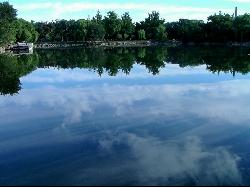
\includegraphics[scale=0.5]{multimedia/pku-lake2.jpg}}	
	\titlepage
\end{frame}

%----------- outline -----------------------------------------------%
\section*{提纲}               	% section后面加*表示不收录到目录中
\begin{frame}{\secname}
 	\tableofcontents            			% 使用这个命令自动生成目录
\end{frame}

%----------- slide item展开-----------------------------------------%
\section{Slide的基本概念}
\begin{frame}{\secname}
  \begin{description}[<+->]				%[<+->]会将列表项依次显示
  \item[何谓幻灯片]
   \li \xiaowu 所谓Slide就是幻灯片的意思,是一种类似照片底片的透明胶片
  \item[幻灯片的作用]
    \fs 帮助演讲者向听众传达文字、图片甚至动画、声音等信息
  \item[幻灯片的优点]
    \kai 省去演讲者抄写时间\\
    表达更准确,更直观\\
    采用计算机,能传达更丰富的内容
  \end{description}
\end{frame}

\section{Beamer效果演示}
%----------- slide 高亮显示------------------------------------------%
\subsection{逐行显示的实现}
\begin{frame}{\subsecname}	
  	\begin{itemize}[<+-|  alert@+>]			%[<+-| alert@+>]高亮显示
  		\item 这一段在第一个Slide上显示,并被加亮
  		\item 这一段在第二个Slide上显示,并被加亮
  		\item 这一段在第三个Slide上显示,并被加亮
  \end{itemize}
\end{frame}

%----------- slide 高亮显示------------------------------------------%
\subsection{字体和色彩的演示}
\begin{frame}{\subsecname}
\textbf<1> 1. \alt<1>{\hei 这是黑体在第一张上}{\fs 这是黑体在第一张上} \\
\textit<2> 2. \song 这是斜体,在第二张上\\
\color<3>[rgb]{1,0,0} 3. 这些文字是在第3张幻灯片上是红色的,其它是黑色的。\\
\only<4>{ 4. 仅在第四张出现。\\}
\alert<4>{4.alert代表红色\\}
\structure<5>{5. structure代表绿色\\}
\alt<6>{6. 仅在第6张}{6. 在1-5张上}
\end{frame}

%----------- slide 换页动态效果---------------------------------------%
\subsection{换页动态效果}
\begin{frame}{\subsecname}
\begin{enumerate}[<+->]
  \item 水平出现效果
    \transblindshorizontal<1>
  \item 竖直出现效果
    \transblindsvertical<2>
  \item 从中心到四角
    \transboxin<3>
  \item 从四角到中心
    \transboxout<4>
  \item 溶解效果
    \transdissolve<5>
  \item Glitter
    \transglitter<6>
  \item 竖直撕开(向内)
    \transsplitverticalin<7>
  \item 竖直撕开(向外)
    \transsplitverticalout<8>
  \item 涂抹
    \transwipe<9>
  \item 渐出
    \transduration<10>{1}
  \end{enumerate}
\end{frame}

%----------- slide 超级链接的实现-------------------------------------%
\subsection{超级链接的实现}
\begin{frame}{\subsecname}
  \hypertarget<1>{jumptofirst}{dd}
  \hypertarget<2>{jumptosecond}{aa}
  \hypertarget<3>{jumptothird}{bb}
  \hypertarget<4>{jumptoforth}{cc}
  \hypertarget<5>{jumptofifth}{ee}
  \begin{itemize}
  \item<1-> 使用 \textbf{hypertarget} 命令添加链接目标
    \hyperlinkframestartnext{\beamerskipbutton{略过}}
  \item<2-> 使用 \textbf{hyperlink} 命令添加链接跳转
  \item<3->
    \hyperlink{jumptoforth}{\beamergotobutton{到第4页}}
  \item<4->
    \beamerbutton{到第公式(\ref{eq1})}
  \item<5->
    \hyperlink{math<5>}{到数学公式页}
  \item<6->
    \hyperlink{jumptofirst}{\beamerreturnbutton{回第1页}}
  \end{itemize}
\end{frame}

%----------- slide 包含视频和音频-------------------------------------%
\subsection{包含视频和音频}
\begin{frame}{\subsecname}
\begin{itemize}
  \item 视频 \\
    \movie[externalviewer,label=mymovie,width=1in,height=0.8in,poster]{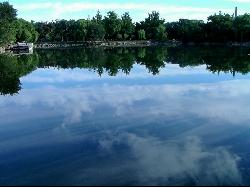
\includegraphics[scale=0.2]{multimedia/pku-lake2.jpg}}{multimedia/movie.avi}
%    \hyperlinkmovie[play]{mymovie}{Play}  
  \item 声音 \\
    \movie[externalviewer,autostart]{这里有一段mp3}{multimedia/turky.mp3}
  \end{itemize}
\end{frame}


%----------- slide 结束---------------------------------------------%
\frame
{
  \frametitle{完}
  \hypertarget{end}{}
}

\end{CJK*}
\end{document}